\documentclass{beamer}
% \documentclass[handout,t]{beamer}
\let\Tiny=\tiny

\batchmode
% \usepackage{pgfpages}
% \pgfpagesuselayout{4 on 1}[letterpaper,landscape,border shrink=5mm]

\usepackage[brazil]{babel}
\usepackage[T1]{fontenc}
\usepackage{amsmath}
\usepackage{amssymb}
\usepackage{color}
\usepackage{subfigure}
%\usepackage{adjustbox}
\usepackage{enumerate}
\usepackage{epsfig}
\usepackage[colorinlistoftodos]{todonotes}
\usepackage{expl3}
\usepackage{supertabular}
\usepackage{float}
\usepackage{graphicx}
\usepackage{ragged2e}
\usepackage{listings}
\usepackage{lmodern}
\usepackage{hhline}
\usepackage[utf8]{inputenc}
\usepackage{bm}
\usepackage{multirow}
\usepackage{pifont}
\usepackage[most]{tcolorbox}
\usepackage{hyperref}
\usepackage{verbatim}
\setbeamertemplate{caption}[numbered]

\newcommand{\revision}[1]{{\color{red}{#1}}}
\newcommand{\rev}[1]{{\color{blue}{#1}}}
\newcommand{\rr}[1]{{\color{orange}{#1}}}
\newcommand{\rer}[1]{{\color{green}{#1}}}
\newcommand{\pu}[1]{{\color{purple}{#1}}}



\usetheme{Berlin}
\usecolortheme{cin}
\setbeamertemplate{headline}{}

% Paginas nos slides
\expandafter\def\expandafter\insertshorttitle\expandafter{%
      \insertshorttitle\hfill%
      \insertframenumber\,/\,\inserttotalframenumber}


% Pazocal
\DeclareMathAlphabet{\pazocal}{OMS}{zplm}{m}{n}

% SpecialCell
\newcommand{\specialcell}[2][c]{%
  \begin{tabular}[#1]{@{}c@{}}#2\end{tabular}}

% Cover ===============================================================
\title[MLG]{Introdução aos Modelos Lineares Clássicos\\
}
\institute[UEPB]{
    \scalebox{2}{
 
\includegraphics[height=.08\textheight]{Marca_UEPB.png}}
}
\author[]{Professor: Pedro Almeida}
\date{{\bf }\\ %{\bf Defesa da Tese de Doutorado}
\vspace{0.1cm}
{\footnotesize Orientadora: Prof.}\\
\vspace{0.1cm}}
\date{}
% End Cover ============================================================


\AtBeginSection[]
{
  \begin{frame}<beamer>
    \frametitle{Roteiro}
    
    \tableofcontents[currentsection]
  \end{frame}
}
\beamerdefaultoverlayspecification{<+->}

\begin{document}

\begin{frame}
\titlepage % Print the title page as the first slide
\end{frame}

\begin{frame}
\frametitle{Roteiro} 
\tableofcontents 
\end{frame}

%----------------------------------------------------------------------------------------
%	PRESENTATION SLIDES
%----------------------------------------------------------------------------------------

%------------------------------------------------
\section{Introdução} 





\frame{\frametitle{Motivação }
\begin{itemize}
\justifying
\item Considere dados extraídos do \rev{censo de 2000} que apresenta para cada unidade da federação o \textbf{número médio de anos de estudo} e a \textbf{renda média mensal dos chefes de domicílio}.

\end{itemize}


\begin{figure}
     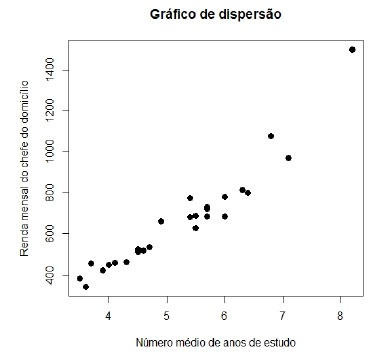
\includegraphics[scale=0.55]{Fig_Dispersao.jpg}
    %\caption{Caption}
    \label{fig:my_label}
\end{figure}

}

\frame{\frametitle{Motivação }
\rer{Queremos responder as seguintes perguntas:}
\begin{itemize}
\justifying
\item <1> A renda mensal dos chefes de domicílio pode ser explicada através
do número médio de anos de estudo destes?
\item <1> Existe um valor numérico que quantifica a relação entre as duas variáveis?
\item <1> Para um valor fixado de anos de estudo de um certo chefe de domicílio, qual será o valor previsto para a renda mensal dos chefes
de domicílio?
\item <1> O quanto da variabilidade da renda mensal pode ser explicado
através do número médio de anos de estudo?

\end{itemize}
}


\frame{\frametitle{Introdução}
\begin{itemize}
\justifying
	\item<1> Existem situações nas quais há interesse em estudar o comportamento conjunto de uma ou mais variáveis;
  \item<1> Em muitos casos, a explicação de um fenômeno de interesse pode estar associado a outros fatores (variáveis) que
contribuem de algum modo para a ocorrência deste fenômeno;
  \item<1> O comportamento conjunto de duas variáveis quantitativas pode ser observado por meio do gráfico de dispersão.
\end{itemize}
}

\frame{\frametitle{Introdução}
\begin{itemize}
\justifying
\item <1> O termo \rev{regressão} foi utilizado pela primeira vez por Galton em 1885, em um estudo que avaliou a relação entre a \revision{altura dos pais e filhos}.

\item <1> O \textbf{objetivo} do estudo foi avaliar como a altura do pai \textbf{influenciava} a altura do filho. Por esse motivo, Galton
denominou de regressão, por existir uma tendência de regressão à média.
\item <1> Em muitas situações, temos interesse em verificar existências de relações entre duas ou mais variáveis. Nesse
sentido, a \textbf{Análise de regressão linear} é uma técnica estatística para modelar e quantificar a relação entre duas ou mais variáveis.


\end{itemize}

}

\section{Tipos de Modelos}


\frame{\frametitle{Tipos de Modelos}
\justifying
Um \textbf{modelo de regressão} é um modelo estatístico em que alguma característica  distribuicional da variável de interesse é afetada por outra(s) variável(is).
  \vspace{0.5cm}
\begin{itemize}
\justifying
     \item<1> É uma das técnicas de modelagem mais usadas;
   
     \item<1> Possui ampla literatura como:
	        \begin{itemize}
              \item<1> \rev{Modelo de Regressão Linear Múltipla}
              \item<1> \rev{Modelo de regressão Não-Linear}
              \item<1> \rev{Modelo Linear Generalizado}
           
         \end{itemize}
\end{itemize}
}


%\frame{\frametitle{Modelo Clássico de Regressão}
%\begin{itemize}
%\justifying
%\item<1> É a técnica mais adequada quando se %deseja estudar o comportamento de uma \textbf{variável dependente} y (variável resposta) em relação a outras \textbf{variáveis independentes} x (variáveis explicativas) que são responsáveis pela variabilidade da variável resposta.
%\end{itemize}
%}

\section{Coeficiente de Correlação}

%%%%%%%%%%%%%%%%%%%%%%%%%%%%%%%%%%%%%%%%ver
\frame{\frametitle{Correlação Linear}

\begin{itemize}
\justifying
	\item<1> No entanto, antes de propor um modelo de regressão é importante verificar o grau de correlação entre as \textbf{variáveis independentes x} e a \textbf{variável resposta y}.
	\item<1> Além disso, nem sempre uma correlação elevada entre variáveis indica que faz sentido propor um modelo de regressão
	     	\begin{itemize}
		           \item<1>\rev{ Ex.: Produção de banana \textit{versus} taxa de natalidade.}
	      \end{itemize}
\item<1> A \textbf{coerência} e \textbf{intuição} do pesquisador é muito importante no momento de propor uma relação entre $x$ e $y$.
\end{itemize}
}

\frame{\frametitle{ Mapas de dispersão e tipos de correlação}

\centering
\begin{figure}[H]
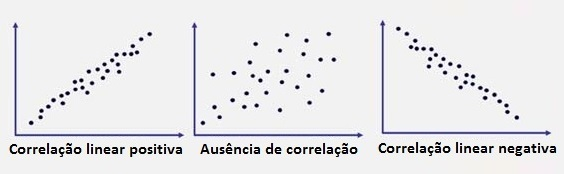
\includegraphics[scale=0.7]{gcor.jpeg}
\begin{center}
{Figura 1: Comportamento do coeficiente de correlação.}
\end{center}
\label{f1}
\end{figure}
}

\frame{\frametitle{Coeficiente de Correlação Linear}
\justifying
Mede a intensidade e a direção da \rev{relação linear} entre duas variáveis.
\scriptsize
\begin{eqnarray*}
\rho(X,Y)&=&\frac{Cov(X,Y)}{\sigma_X \cdot \sigma_Y}\\
&=&\frac{n\displaystyle\sum _{i=1} ^{n} x_i y_i- \sum _{i=1} ^{n} x_i \sum_{i=1} ^{n}y_i}{\sqrt{n \displaystyle\sum _{i=1} ^{n} x_{i} ^{2}-\left(\sum _{i=1} ^{n} x_{i} \right)^2} \sqrt{n\displaystyle\sum _{i=1} ^{n} y_{i} ^{2} - \left(\sum _{i=1} ^{n} y_i\right)^2}}, \quad i=1, \ldots, n.
\end{eqnarray*}
\small
em que $n$: tamanho da amostra; $y$: variável dependente; $x$: variável independente; $\sigma_X$ e $\sigma_Y$ é o desvio de X e Y, respectivamente; ${\mbox{Cov}(X,Y)}$ é a covariância entre duas variáveis.
}


\frame{\frametitle{Coeficiente de Correlação Linear}
\justifying

\centering
\begin{figure}[H]
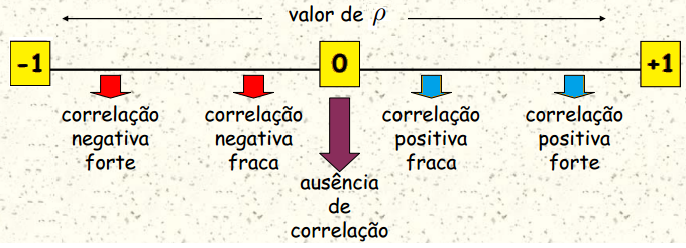
\includegraphics[scale=0.5]{corr.jpeg}
\begin{center}
{Figura 2: Variação do coeficiente de correlação.}
\end{center}
\label{f22}
\end{figure}

\begin{itemize}
    \item <1> Se $\rho = 1$ implica correlação \textbf{linear positiva e perfeita};
    \item <1>  Se $\rho = -1$ implica correlação \textbf{linear negativa e perfeita};
    \item <1>  Se $\rho = 0$ \textbf{inexistência} de correlação linear.
\end{itemize}

}

%\frame{\frametitle{Exemplo 1}
%\justifying
%Considere uma amostra de dez dos 98 alunos de uma Faculdade A, e as notas obtidas foram (CRESPO, 1993)
%\begin{table}
%\centering
%\label{t1}
%\begin{tabular}{c|c|c}
%\hline
%\multicolumn{3}{c}{Notas}\\
%\hline
%N°  & Matemática & Estatística \\\hline
%01&5&6\\
%08&8&9\\
%24&7&8\\
%38&10&10\\
%44&6&5\\
%58&7&7\\
%59&9&8\\
%72&3&4\\
%80&8&6\\
%92&2&2\\
%\hline
%\end{tabular}
%\end{table}
%}

%\frame{\frametitle{Exemplo 1}
%\justifying
%\centering
%\begin{figure}[H]
%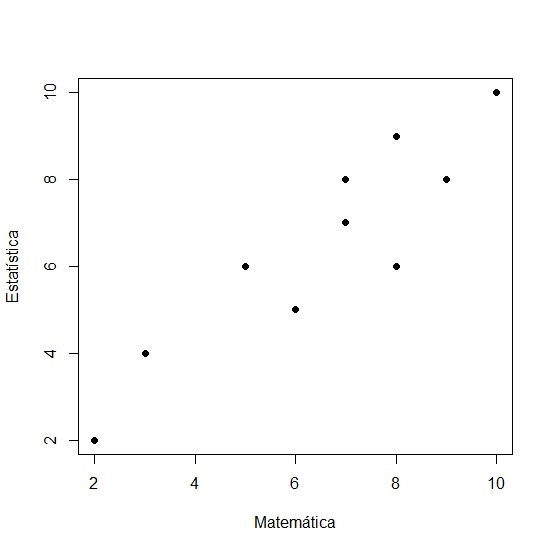
\includegraphics[scale=0.45]{ex1.jpeg}
%\begin{center}
%{Figura 3: Dispersão dos dados.}
%\end{center}
%\label{f3}
%\end{figure}
%}

%\frame{\frametitle{Exemplo 1}
%\justifying
%\scriptsize
%\begin{table}
%\centering
%\label{t19}
%\begin{tabular}{c|c|c|c|c}
%\hline
% Matemática ($x_i$)& Estatística ($y_i$) &$x_{i}y_{i}$ & $ x_{i} ^{2}$ & $y_{i}^{2}$ \\\hline
%5&6&30&25&36\\
%8&9&72&64&81\\
%7&8&56&49&64\\
%10&10&100&100&100\\
%6&5&30&36&25\\
%7&7&49&49&49\\
%9&8&72&81&64\\
%3&4&12&9&16\\
%8&6&48&64&36\\
%2&2&4&4&4\\\hline
%$\sum =65$ & $\sum =65 $ & $\sum =473$ & $\sum =481$& $\sum =475$\\ 
%\hline
%\end{tabular}
%\end{table}

%\begin{equation*}
%\rho= \frac{10 \times 473 -65 \times 65}{\sqrt{(10 \times 481-65^{2})(10 \times 475-65^{2})}}=\frac{505}{554,18}=0,911
%\end{equation*}
%\justifying

%Logo, o resultado indica uma correlação linear positiva entre as duas variáveis. \rev{Faça em R!}
%\todo{This is a comment that will appear in the margin}
%}

\frame{\frametitle{Modelo de Regressão Linear Simples (MRLS)}

\begin{itemize}
\justifying
	\item<1> Seja $Y$ uma variável resposta, e seja $X$ uma variável denominada de  regressora (FREIRE et al, 2008).
	
	\item<1> O MRLS descreve a variável $Y$ como uma soma de uma quantidade determinística e uma quantidade aleatória.
		\begin{itemize}
		  \item<1> Parte determinística: uma reta em função de $X$.
		  \item<1> Parte aleatória: denominada de erro.
	  \end{itemize}
\end{itemize}
}

\frame{\frametitle{Modelo de Regressão Linear Simples (MRLS)}
\justifying
O modelo de regressão é chamado de \rev{simples} quando envolve uma relação causal entre duas variáveis.
\begin{equation*}
\label{eq1}
Y=\beta_0 + \beta_1X+ \epsilon,
\end{equation*}

\begin{itemize}
\justifying
	\item<1>  $\beta_0$ e $\beta_1$ são os parâmetros da regressão que são
desconhecidos e devem ser estimados;
	\item<1> $\epsilon$, é o erro que é uma variável aleatória não-observável, em que é
   suposto que \textbf{E($\epsilon) = 0$} e \textbf{Var($\epsilon) = \sigma^2$}.
   
   \end{itemize}
}



\frame{\frametitle{Modelo de Regressão Linear Simples (MRLS)}
Suposições
\begin{description}
\justifying
	\item<1>[S0] O modelo  está correto;
	\item<1>[S1] $\mbox{E}(\epsilon_i)=0 \,\,\forall _i$; 
	\item<1>[S2] $\mbox{Var}(\epsilon_i)= \sigma^2\,\,\forall _i \,\,(0< \sigma ^2<\infty)$;
	\item<1>[S3] $\mbox{Cov}(\epsilon_i,\epsilon_s)=0 \,\,\forall\, i \,\, \neq s$;
	\item<1>[S4] $x$ assume pelo menos dois valores;
	\item<1>[S5] Normalidade.
\end{description}
}

\frame{\frametitle{Modelo de Regressão Linear Simples (MRLS)}
\justifying
Considere o modelo de regressão linear simples. Então a distribuição de $Y$, correspondente ao valor prefixado, x, de $X$, é dado por:

\begin{equation*}
Y \sim \mathcal{N}(\beta_0 +\beta_1 x; \sigma^2).
\end{equation*}
\textbf{Prova:}\\
\begin{eqnarray*}
I\!\!E(Y|x)&=& I\!\!E \left(\beta_0+ \beta_1 x+ \epsilon \right)\\
& = & I\!\!E \left(\beta_0+ \beta_1 x \right)+ I\!\!E (\epsilon)\\
&=& \beta_0 + \beta_1 x +0.
\end{eqnarray*}
}

\frame{\frametitle{Modelo de Regressão Linear Simples (MRLS)}
\justifying

\begin{eqnarray*}
\mbox{Var}(Y|x)&=& \mbox{Var} \left(\beta_0+ \beta_1 x+ \epsilon \right)\\
&=& \mbox{Var} \left(\beta_0+ \beta_1 x \right)+ \mbox{Var} (\epsilon)\\
&=& 0 + \sigma^2\\
&=& \sigma^2.
\end{eqnarray*}


}


\frame{\frametitle{Modelo de Regressão Linear Simples (MRLS)}
\justifying
Expressando este modelo usando notação matricial. Sejam os vetores

\begin{table}[H]
\centering
\label{t111}
\begin{tabular}{ccc}

$\bf{Y} = \left[ \begin{array}{c} y_1 \\ y_2\\ \vdots  \\ y_n \\  \end{array} \right],$& $\bf{\beta} = \left[ \begin{array}{c} \beta_0 \\ \beta_1\\ \end{array} \right] \text{e} $&${\bf{\epsilon}} = \left[ \begin{array}{c} \epsilon_1 \\ \epsilon_2\\ \vdots  \\ \epsilon_n \\  \end{array} \right].$\\
\end{tabular}
\end{table}
E seja a matriz $X$:

$$
\bf{X} = \left[\begin{array}{cc} 1& x_{1}\\ 1& x_{2}\\ \vdots& \vdots\\ 1 & x_n\\  \end{array} \right].
$$
}

\frame{\frametitle{Modelo de Regressão Linear Simples (MRLS)}
\justifying
Então,

\begin{equation*}
\tiny{
\bf{{X}} {\beta} + \epsilon= \left[\begin{array}{cc} 1& x_{1}\\ 1& x_{2}\\ \vdots& \vdots\\ 1 & x_n\\  \end{array} \right]  \left[ \begin{array}{c} \beta_0 \\ \beta_1\\ \end{array} \right]+ \left[ \begin{array}{c} \epsilon_1 \\ \epsilon_2\\ \vdots  \\ \epsilon_n \\  \end{array} \right]= \left[ \begin{array}{c} 
\beta_0+ \beta_1 x_1 + \epsilon_1\\ \beta_0+ \beta_1 x_2 + \epsilon_2\\ \vdots\\ \beta_0+ \beta_1 x_n + \epsilon_n \end{array} \right]= \left[ \begin{array}{c} y_1 \\ y_2\\ \vdots  \\ y_n \\  \end{array} \right]={y}}
\end{equation*}
}

\frame{\frametitle{Modelo de Regressão Linear Simples (MRLS)}
\justifying
O vetor aleatório ${\epsilon}$ é composto de variáveis independentes, com distribuição $\mathcal{N} (0; \sigma^2)$. Desta forma, o vetor de esperanças dos elementos de ${\epsilon}$ é o vetor nulo de dimensão $n$ e a matriz, cuja diagonal é formada pelas variâncias e os demais elementos são as covariâncias, logo a \textbf{matriz de variância e covariância} é dado por

$$
\left[\begin{array}{ccccc} \sigma^2&0&0& \ldots & 0\\ 0&\sigma^2&0& \ldots & 0\\ \vdots &\vdots &\vdots  &\ldots &\vdots \\ 0&0&0&0& \ldots \sigma^2 \\ \end{array} \right]=\sigma^2  I,
$$
sendo ${I}$ a matriz identidade de ordem $n$.
}


\section{Estimação  dos Parâmetros}


\frame{\frametitle{Método dos Mínimos Quadrados}
\begin{itemize}
    \justifying
		\item<1> A estimação de $\beta_0$ e $\beta_1$ pode ser feita pelo \textbf{Método dos Mínimos Quadrados}, que não requer qualquer hipótese sobre a distribuição das componentes do vetor y, e consiste em minimizar.
\end{itemize}

\begin{equation*}
S(\beta_0, \beta_1) = \displaystyle \sum _{i=1} ^{n} \left[y_i-\left(\beta_0 + \beta_1 x_i \right) \right]^{2} = \displaystyle \sum _{i=1} ^{n} {\epsilon _i}^2.
\end{equation*}

\justifying
em que $y_i$ e $x_i$ são os valores observados de $Y_i$ e $X_i$, respectivamente, com $i = 1,2, \cdots,n.$
Ao minimizar $S(\beta_0; \beta_1)$ com respeito a $\beta_0$ e $\beta_1$, estaremos minimizando
a informação perdida ao utilizar o MRLS para modelar Y.
}


\frame{\frametitle{Método dos Mínimos Quadrados}
\justifying
Para encontrar esse mínimo precisamos obter as seguintes derivadas parciais:

	\begin{equation*}
	\frac{\partial}{\partial \beta_0} \displaystyle \sum _{i=1} ^n \left[ y_{i} - \left(\beta_0 + \beta_1 x_{i} \right)\right]^2
	\end{equation*}
	
	\begin{equation*}
	\frac{\partial}{\partial \beta_1} \displaystyle  \sum _{i=1} ^n [y_{i} - (\beta_0+ \beta_1 x_{i})]^2
	\end{equation*}
	
	}


\frame{\frametitle{Método dos Mínimos Quadrados}
\justifying
Denominado por ${\hat{\beta}_0}$ e ${\hat{\beta}_1}$ os valores que minimizam a função temos

\begin{equation*}
-2 \displaystyle  \sum _{i=1} ^n \left[y_{i} - \left( \hat\beta_0 + \hat\beta_1 x_i \right) \right]=0
\end{equation*}

\begin{equation*}
-2 \displaystyle  \sum _{i=1} ^n \left[y_i- \left( \hat\beta_0 + \hat\beta_1 x_{i} \right) \right] x_{i} =0,
\end{equation*}
denominado sistema de equações normais.
\vspace{0.5cm}

\rev{Para garantir que $(\hat{\beta_0}; \hat{\beta_1})$ é de fato ponto de mínimo da função $(\beta_0; \beta_1)$,
precisamos obter a matriz de segundas derivadas e mostrar que está é não-negativa definida. \revision{Prove!}}
}


\frame{\frametitle{Ajuste e Predição}
Logo após alguma álgebra
$$
\hat{\beta_0} =\bar{y}-\hat{\beta_1} x
$$
$$
\hat {\beta_1}=\frac{\displaystyle  \sum _{i=1} ^n (y_i - \bar{y})(x_i-\bar{x})}{\displaystyle  \sum _{i=1} ^n  (x_i- \bar{x})^2}
=\frac{\displaystyle  \sum _{i=1} ^n y_i(x_i- \bar{x})}{\displaystyle  \sum _{i=1} ^n (x_i - \bar{x})^2}
$$
Assim, para prever valores de $Y$ para valores fixados de $X$, utiliza-se
$$
\hat{y}_0 = \hat{\beta}_0 + \hat{\beta}_1 x_0;
$$
\justifying
em que $x_0$ é um valor fixado para a covariável e $\hat{y}_0$ é o valor previsto para a variável resposta.
O valor fixado para $x_0$ deve estar próximo aos limites do valores observados de $X$ da amostra utilizada para estimar os coeficientes da
regressão.


}


\frame{\frametitle{Interpretação dos Coeficientes Estimados}
\justifying
Para \rev{interpretar o coeficiente estimado $\hat{\beta}_0$}, tome $x_i = 0$. Então, o MRLS ajustado é 

$$
\hat{\mu}_i = \hat{y}_i= \beta_0
$$
\justifying
- Note que $\hat{\beta}_0 $ é o ponto onde a reta de regressão ajustada \textbf{intercepta o eixo x}.\\
\vspace{0.5cm}
- $\hat{\beta}_0$ é uma estimativa para a média da variável resposta quando a covariável assume valor zero. 

\vspace{0.5cm}




}


\frame{\frametitle{Exemplo 2}
\justifying
Para \rev{interpretar $\hat{\beta}_1$}, considere o aumento de uma unidade no valor da
covariável, isto é, $x_0 = x + 1$. Então,

\begin{eqnarray}\nonumber
\hat{y}& =& \hat{y}(x') - \hat{y}(x)\\ \nonumber
&=& \hat{\beta}_0 + \hat{\beta}_1x'- \hat{\beta}_0 - \hat{\beta}_ 1 x\\ \nonumber
&=& \hat{\beta}_0 + \hat{\beta}_1(x + 1) - \hat{\beta}_0 -\hat{\beta}_1 x\\\nonumber
&=& \hat{\beta}_1\\\nonumber
\end{eqnarray}

Logo, além de $\hat{\beta}_1$ ser o coeficiente angular da reta de regressão, este, também, é o quanto o valor da \rev{média estimada de $Y$ varia quando aumentamos uma unidade da variável $X$}.
}

\frame{\frametitle{Exemplo 2}
\justifying
Encontre a reta de mínimos quadrados  e os resíduos para os seguintes pares de valores (FREIRE et al, 2008):

\scriptsize
\begin{table}
\centering
\label{t11}
\begin{tabular}{|c|cccccc|}
\hline
x&1& 1& 2& 2& 3& 3\\
y& 1& 3& 1& 3& 1& 3\\
\hline
\end{tabular}
\end{table}
\textcolor {red} {Solução:}
\scriptsize
\begin{table}
\centering
\label{t122}
\begin{tabular}{|ccccc|cc|}
\hline
&x&y& $x^2$& xy& $\hat{y}$& $\epsilon=y- \hat{y}$\\ \hline
&1&1& 1&1& 2& $-1$\\
&1&3& 1& 3& 2&1\\
&2&1 &4& 2&2& $-1$\\
&2&3& 4& 6& 2& 1\\
&3&1& 9& 3& 2& $-1$\\
&3&3& 9& 9& 2& 1\\\hline
soma&12&12& 28& 24& 12& 0\\
\hline
\end{tabular}
\end{table}
}

\frame{\frametitle{Exemplo 2}
\justifying

Usando a soma das 4 primeiras colunas da tabela, obtemos

$$
\bar{x}=\frac{12}{6} \quad \bar{y}=\frac{12}{6}=2,
$$

$$
\hat{\beta_1}=\frac{24-\frac{1}{6}(12 \times 12)}{28-\frac{1}{6}(12)^2}=0 \quad \hat{\beta_0}=2-0(2)=2
$$

portanto, a reta de mínimos quadrados é $\hat {y}= 2.$
}

\frame{\frametitle{Propriedades do Ajuste de Mínimos Quadrados}
\scriptsize
\begin{itemize}
\item<1> $\displaystyle  \sum _{i=1} ^n y_i= \displaystyle  \sum _{i=1} ^n \hat{y_i}$\\
\begin{center}
\scriptsize{
Prova:$\quad \quad \quad \quad \displaystyle  \sum _{i=1} ^n y_i - n\hat{\beta_0} - \hat{\beta}_1 \displaystyle  \sum _{i=1} ^n x_i=0$\\
$ \rightarrow \displaystyle  \sum _{i=1} ^n y_i - \displaystyle  \sum _{i=1} ^n \underbrace{(\hat{\beta}_0 + \hat{\beta}_1 x_i )}_{\hat{y}_i}=0.$}
\end{center}
\item<1> $\displaystyle  \sum _{i=1} ^n e_i= 0$
\begin{center}
\scriptsize{
Prova:$ \quad \quad \quad \quad \displaystyle  \sum _{i=1} ^n y_i - \displaystyle  \sum _{i=1} ^n \hat{y_i}=0$\\
$ \rightarrow \displaystyle  \sum _{i=1} ^n \underbrace{(y_i -\hat{y_i})}_{e_i}=0.$\\
}
\end{center}
\end{itemize}
}

\frame{\frametitle{Propriedades do Ajuste de Mínimos Quadrados}
\scriptsize

\begin{itemize}
\item<1> $\displaystyle  \sum _{i=1} ^n x_i e_i=0$
\begin{center}
Prova:$\quad \quad  \quad   \quad \displaystyle  \sum _{i=1} ^n x_i y_i - \hat{\beta_0}\displaystyle  \sum _{i=1} ^n x_i -\hat{\beta_1} \displaystyle  \sum _{i=1} ^n x_i ^2=0$\\
$\rightarrow \displaystyle  \sum _{i=1} ^n x_i \underbrace{(y_i - \hat{\beta_0} - \hat{\beta_1}x_i)}_{e_i}=0.$\\
\end{center}
\item<1> $\displaystyle  \sum _{i=1} ^n \hat{y_i} e_i=0$
\begin{center}
Prova:$\quad \quad \quad \quad \displaystyle  \sum _{i=1} ^n \hat{y_i}{e_i}=   \displaystyle  \sum _{i=1} ^n (\hat{\beta_0} -\hat{\beta_1}x_i)e_i$\\
$=\hat{\beta_0} \underbrace{\displaystyle  \sum _{i=1} ^n e_i}_{0}- \hat{\beta_1}\underbrace{\displaystyle  \sum _{i=1} ^n x_i e_i}_{0}.$
\end{center}
\end{itemize}
}


\frame{\frametitle{Estimadores de Mínimos Quadrados para o MRLS}

\begin{itemize}
\item<1> $\mbox{E}(\hat {\beta_1})= \beta_1$ e $\mbox{E}(\hat {\beta_0})= \beta_0$\\

\item<1> $\mbox{Var}(\hat{\beta_1})=\frac{\sigma^2}{\displaystyle  \sum _{i=1} ^n (x_i -\bar{x})^2}$\, e \,$\mbox{Var}(\hat{\beta_0})=\sigma^2\left[\frac{1}{n}+\frac{\bar{x}^2}{\displaystyle  \sum _{i=1} ^n (x_i- \bar{x})^2}\right]$
\end{itemize}
}

\frame{\frametitle{Estimadores de Mínimos Quadrados para o MRLS}
\justifying

Precisamos estimar mais um parâmetro \rev{``a variância do erro, $\sigma^2"$}, o qual representa a distorção da reta. Um estimador não-viesado de $\sigma^2$ para o modelo de regressão simples é dado por 

$$
\hat{\sigma^2}=\frac{\displaystyle  \sum _{i=1} ^n (y_i - \hat{y}_i)^2}{n-2}
$$

sob o MRLS,  $\frac{(n-2) \hat{\sigma^2}}{\sigma^2} \sim \mathcal{X}^2 _{(n-2)}$.

}


\frame{\frametitle{Decomposição da Soma de Quadrados Total}
\begin{itemize}
\justifying
\item<1> Técnica mais usada para verificar a adequação do ajuste do modelo de regressão a um conjunto de dados, baseada na seguinte identidade 

\end{itemize}
\begin{eqnarray*}
\displaystyle  \sum _{i=1} ^n (y_i - \bar{y})^2 &=& \displaystyle  \sum _{i=1} ^n(\hat{\mu}_i - \bar{y})^2 + \displaystyle  \sum _{i=1} ^n (y_i-\hat{\mu}_i)^2\\
\end{eqnarray*}

\quad \quad \quad \quad \quad \quad SQT \quad \quad = \quad \quad \quad SQE \quad \quad +\quad \quad \quad SQR

}


\frame{\frametitle{Coeficiente de determinação - $R^2$}
\justifying
O \rev{coeficiente de correlação} múltipla de Pearson (ou coeficiente de determinação) ${R^2}$  expressa o quanto o modelo explica a variabilidade total da variável y.
	
	
$$
R^2=\frac{SQE}{\text{SQT}}
$$

\begin{itemize}
\justifying
	\item<1> O \rev{coeficiente $R^2$} é interpretado como a proporção da variação de $Y$ que é explicada pela covariável X. $( \in (0,1))$
	\item <1> \revision{Finalidade:} Medir o poder de explicação de um modelo.
\end{itemize}
}

\frame{\frametitle{Análise dos Resíduos}
\justifying
\begin{itemize}
\item <1> resíduos ordinários;
\item <1> resíduos padronizados.
\end{itemize}

\begin{figure}
    \centering
    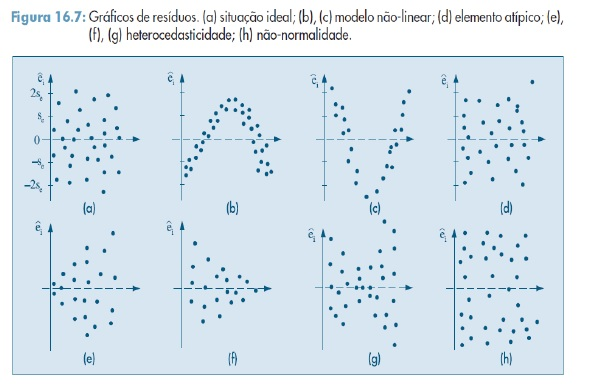
\includegraphics[scale=0.5]{Fig_Residuo.jpg}
        \label{fig:my}
\end{figure}
\center{\textbf{Fonte:} MORETTIN e BUSSAB (2010).}

}

\frame{\frametitle{Tabela ANOVA}
\justifying
A tabela da \textbf{ANOVA} é usada para testar a adequação global do modelo de regressão
\scriptsize
\begin{table}
\centering
\label{t12}
\begin{tabular}{|ccccc|}
\hline
Efeito&Soma de & G.L. & Média de &Estatística \\
& Quadrados&& Quadrados&\\ \hline \hline
Regressão&SQE&$1$& MQE=SQE/($1$)& F=MQE/MQR\\
Residual&SQR& $n-2$&MQR= SQR/($n-2$)& \\ \hline
Total&SQT& $n-1$&&\\ \hline
\end{tabular}
\end{table}
\small
%As somas SQE e SQR tem distribuições $\sigma^2 \mathcal{X}^2_{1} $ e $\sigma^2 \mathcal{X}^2_{n-2}$, respectivamente. 
}
\frame{\frametitle{Teste F- Adequação Global}
\begin{itemize}
	\item<1> Hipóteses:\\
	
	\begin{center}
		$H_0: \beta_1 = 0$\\
	$H_1:  \beta_1 \neq 0$ 
\end{center}
	\item<1> Estatística de Teste\\
	
	\begin{center}
	F=MQE/MQR
	\end{center}
	\item<1> \textbf{Se ${F} > {F_{1, n-2}} (\alpha)$ rejeita ${H_0}$}, logo o efeito global de pelo menos algumas variáveis presentes na matriz X explica a variabilidade de y.
	\end{itemize}
}


\frame{\frametitle{Teste F- Adequação Global}
\begin{itemize}
\justifying
	\item<1> A estatística do teste \textcolor{red}{F} representa o quociente entre \textbf{SQE} e \textbf{SQR} e têm distribuição $ \mathcal{X}^2$, pelos respectivos G.L., logo temos que

$$
F \sim F_{1, \, n-2},
$$
que representa o valor de uma distribuição F-Snedecor com $1$ e $n-2$  graus de liberdade, ao nível de significância $\alpha$.
\end{itemize}
}

\frame{\frametitle{Seleção das Variáveis Explicativas}

\begin{itemize}
\justifying
	\item<1> O \textbf{Teste F} permite apenas inferir que algumas variáveis explicativas são realmente importantes (mas não sabemos quais!). 
	\item<1> O \textbf{Teste t} permite selecionar as variáveis independentes (explicativas) que são significativas para o modelo.
\end{itemize}
}

\frame{\frametitle{Seleção das variáveis explicativas- Teste t}

\begin{itemize}
\justifying
	\item<1> Obter um modelo parcimonioso; 
	\item<1> Eliminar variáveis que tem pouca ou nenhuma contribuição na variabilidade da variável dependente y.
	\item<1> Hipóteses:\\
	
	\begin{center}
	$H_0: \beta_0= 0$\\
		$H_1: \beta_0 \neq 0.$
\end{center}
\end{itemize}
}


\frame{\frametitle{Seleção das Variáveis Explicativas- Teste t}

\begin{itemize}
\item<1> Estatística do Teste\\
$$
T= \frac{\hat{\beta}_1}{\sqrt\frac{\hat{\sigma^2}}{\displaystyle  \sum _{i=1} ^n (x_i - \bar{x})^2}}
$$
\justifying
\item<1> \textbf{Se} ${T < t_{n-2}} (\alpha/2)$ \textbf{não rejeita} ${H_0}$, logo a variável independente $X$ não é significativa para explicar a variabilidade da resposta.
\end{itemize}
}

\frame{\frametitle{Exemplo 3}

Comandos utilizados para o ajuste do modelo de regressão liner simples no \textcolor{blue}{\textit{software} R}.
\begin{verbatim}

\#dados\\
x=c(5,8,7,10,6,7,9,3,8,2)\\
y=c(6,9,8,10,5,7,8,4,6,2)\\

\#Ajuste do modelo
ajuste=lm(y \sim x)\\
summary(ajuste)\\
\end{verbatim}
}


\frame{\frametitle{Exemplo 3}
\centering
\begin{figure}[H]
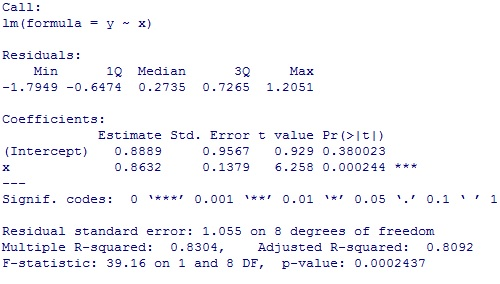
\includegraphics[scale=0.7]{RR.jpg}
\begin{center}
{Figura 4: Resultados do ajuste obtidos no R.}
\end{center}
\label{f2}
\end{figure}
}





\begin{frame}
\frametitle{Referências}
\footnotesize{
\begin{thebibliography}{99} % Beamer does not support BibTeX so references must be inserted manually as below
\justifying


\bibitem <1> []{}Paula, Gilberto Alvarenga. (2004) Modelos de regressão: com apoio computacional. São Paulo: IME-USP.

\end{thebibliography}
}




\end{frame}

%----------------------------------------------------------------------------------------

\end{document}